\subsection{Aufbau des Nao}
%* zu softbank robotics
%* allgemeines zur größe, zu den freiheitsgraden und den Sensoren
%* Genaueres zu den Sensoren, die gemessen wurden
%* Grenzen des Naos
Nao ist ein $574 \unit{mm}$ großer humanoider Roboter ursprünglich entwickelt von dem französischen Unternehmen Aldeberan Robotics, welche 2015 von Softbank Group aufgekauft \cite{aldebaran_to_softbank} und in Softbank Robotics umbenannt wurde. 

\begin{wrapfigure}{r}{0.5\linewidth}
	\vspace{-0.5cm}
	\centering
	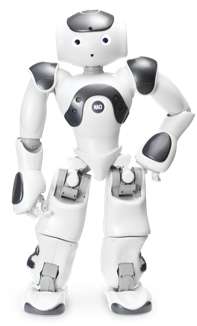
\includegraphics[width=\linewidth]{Bilder/naov6.png}
	\caption{Nao}
	%\cite[in /kinematics-data/joints]{nao_docu_dev_guide}}
	\label{nao_v6}
	\vspace{-0,5cm}
\end{wrapfigure}

\begin{figure}[htb]
	\centering
	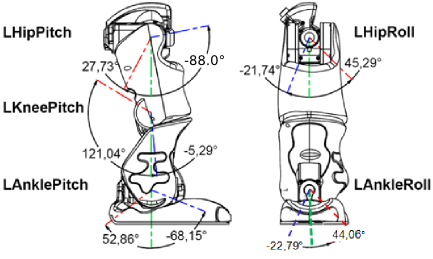
\includegraphics[width=0.7\linewidth]{Bilder/hardware_llegjoint.png}
	\caption{Position und mögliche Winkel der Aktoren des linken Beins. \cite[in /kinematics-data/joints]{nao_docu_dev_guide}}
	\label{hardware_llegjoint}
\end{figure}
\begin{figure}[htb]
	\centering
	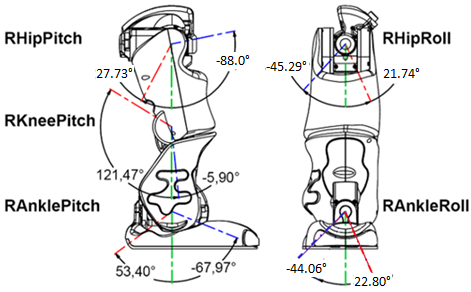
\includegraphics[width=0.7\linewidth]{Bilder/hardware_rlegjoint.png}
	\caption{Position und mögliche Winkel der Aktoren des rechten Beins. \cite[in /kinematics-data/joints]{nao_docu_dev_guide}}
	\label{hardware_rlegjoint}
\end{figure}

\begin{figure}[htb]
	\centering
	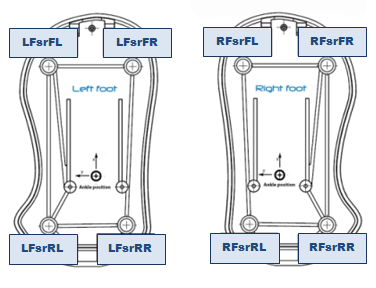
\includegraphics[width=0.6\linewidth]{Bilder/hardware_semelles.png}
	\caption{Sensoren am Fuß. %\cite[in /kinematics-data/joints]{nao_docu_dev_guide}
	}
	\label{hardware_semelles}
\end{figure}

\subsection{Magneto-aktive Polymere}\label{kap_MAP}
%	 woher kommt der begriff, was ist es
%	 woher bestand die bisherige Forschung, warum ist es interessant
\subsubsection{Begriffserklärung und Eigenschaften}
Der Begriff magneto-aktive Polymere (MAP) schließt eine Gruppe von intelligenten, auf Felder ansprechende Materialien ein, welche typischerweise Kombinationen aus einer weichen, polymetrischen Grundlage und magnetisch aktiven Partikeln sind. Diese Partikel werden während dem Vernetzungsprozess des Polymers in dieses eingebettet. 

Die wesentlichen Verhaltensweisen, die MAP in der heutigen Zeit attraktiv für seine Verwendung gemacht hat, wurde bereits in den 80ger Jahren von Rigbi und Jilken \cite{Rigbi1} sowie Rigbi und Mark \cite{Rigbi2} beschrieben. Ein Jahrzehnt später wurde eine genauere Analyse zum ersten Mal von Ginder und Jolly et al. \cite{ginder} veröffentlich. 
Diese kombinierten, aus mehreren Kompontenten bestehenden Materialen stechen durch zwei Schlüsseleigenschaften heraus. 
Zum einen ist es das magnetostriktive Verhalten, bei dem es sich um das Phänomen der Verformung eines Materials handelt, welches durch ein Magnetfeld hervorgerufen wird. \cite{gulley}
Zum anderen sind es die leicht veränderbaren Materialeigenschaften wie Elasizität und Dämpfungsfaktor, welche hauptsächlich mit der Mikrostruktur des Grundlagenmaterials zusammenhängt. \cite{Varga1} \cite{Varga2}

Außerdem ist entscheidend, wie die magnetischen Partikel in das Polymer eingebettet werden. Je nachdem ob während des Vernetzungsprozesses ein Magnetfeld wirkt, können sich die Partikel kettenförmig ausrichten und dadurch dem MAP eine anisotropisches Verhalten zuführen. Isotropisches MAP hingegen enthält keine gerichteten Partikel. Diese verschiedenen Ausrichtungsarten können sowohl die Steifigkeit verändern als auch bestimmen, ob das MAP in einem Magnetfeld ausgedehnt oder zusammengedrückt wird. 

%\subsubsection{Herstellung}

\subsubsection{Anwendungsbereiche}
Weiche, mit einem Feld manipulierbare, Polymere haben diverse Anwendungsbereiche in akademischen und industierellen Bereichen. Angefangen von anpassungsfähiger Vibrationsabsortion in der Luftfahrt und Automobilindustrie durch das Einsetzen durch Scherung (cite 175,114) Windung(202) und Kompression bzw. Elongation(246) und vibrationsisolatoren (cite 174) sowie Sensoren (174,334), Ventile und Aktoren (55,254) und anpassungsfähige Sandwichartige Strukturen (575,576,560) bis hin zur Anwendung in der Bionik wie zum beispiel durch Mikro- und Nanoroboter und Schwimmroboter (438,561.329.219), Schlauchradpumpen (152) und Erschütterungsisolatoren (308).

Desweiteren wird die Verhärtung bei Anlegen eines Magnetfeldes für Greifer genutzt (cite suchen), ebenso wird der 3D Druck von magneto-aktiven Polymeren (cite von uns) wird bereits erforscht.

\subsection{Verwendete Software}
	
%%% Local Variables:
%%% mode: latex
%%% TeX-master: "main"
%%% End: